\documentclass[aspectratio=169]{beamer}

\usepackage[utf8]{inputenc}
\usepackage[spanish]{babel}
\usepackage{graphicx}
\usepackage{booktabs}
\usepackage{ragged2e}
\usepackage{minted}
\usepackage{xcolor}
\usepackage{tikz}
\usepackage{algorithm}
\usepackage{algorithmic}
\usepackage{minted}
\usepackage{listings}
\usepackage{tikz}
\usetikzlibrary{arrows.meta,positioning,fit,shapes.symbols}
\usetikzlibrary{arrows,shapes}
\definecolor{LightGray}{gray}{0.975}
\definecolor{links}{HTML}{2A1B81}
\hypersetup{colorlinks,linkcolor=,urlcolor=blue}

\usefonttheme{serif}

\title[Performance]{Database Administration}
\subtitle{Lecture 07: Performance Tuning.}
\author{Valeja \& Gonzales.}
\date{\today}

% Remove navigation symbols...
\setbeamertemplate{navigation symbols}{}

\defbeamertemplate*{footline}{shadow theme}{
    \leavevmode
    \hbox{
        \begin{beamercolorbox}[
                wd =        0.33\paperwidth,
                ht =        2.5ex,
                dp =        1.125ex,
                leftskip =  0.3cm plus1fil,
                rightskip = 0.3cm
            ]{author in head/foot}
            \flushleft DBA
        \end{beamercolorbox}
        \begin{beamercolorbox}[
                wd =        0.33\paperwidth,
                ht =        2.5ex,
                dp =        1.125ex,
                leftskip =  0.3cm plus1fil,
                rightskip = 0.3cm
            ]{author in head/foot}
            \insertshorttitle
        \end{beamercolorbox}
        \begin{beamercolorbox}[
                wd =        0.33\paperwidth,
                ht =        2.5ex,
                dp =        1.125ex,
                leftskip =  0.3cm plus1fil,
                rightskip = 0.3cm
            ]{title in head/foot}
            \hfill \insertframenumber\,/\,\inserttotalframenumber%
        \end{beamercolorbox}
    }
}

\AtBeginSection[]
{
     \begin{frame}<beamer>
     \frametitle{Plan}
     \tableofcontents[currentsection]
     \end{frame}
}

\newcommand{\toRight}[1]{
    \begin{FlushRight}
        {\tiny #1}
    \end{FlushRight}
} % Align to right

\begin{document}

\frame{\titlepage}

\begin{frame}{Database Administration: Performance Tuning.}
    \centering
    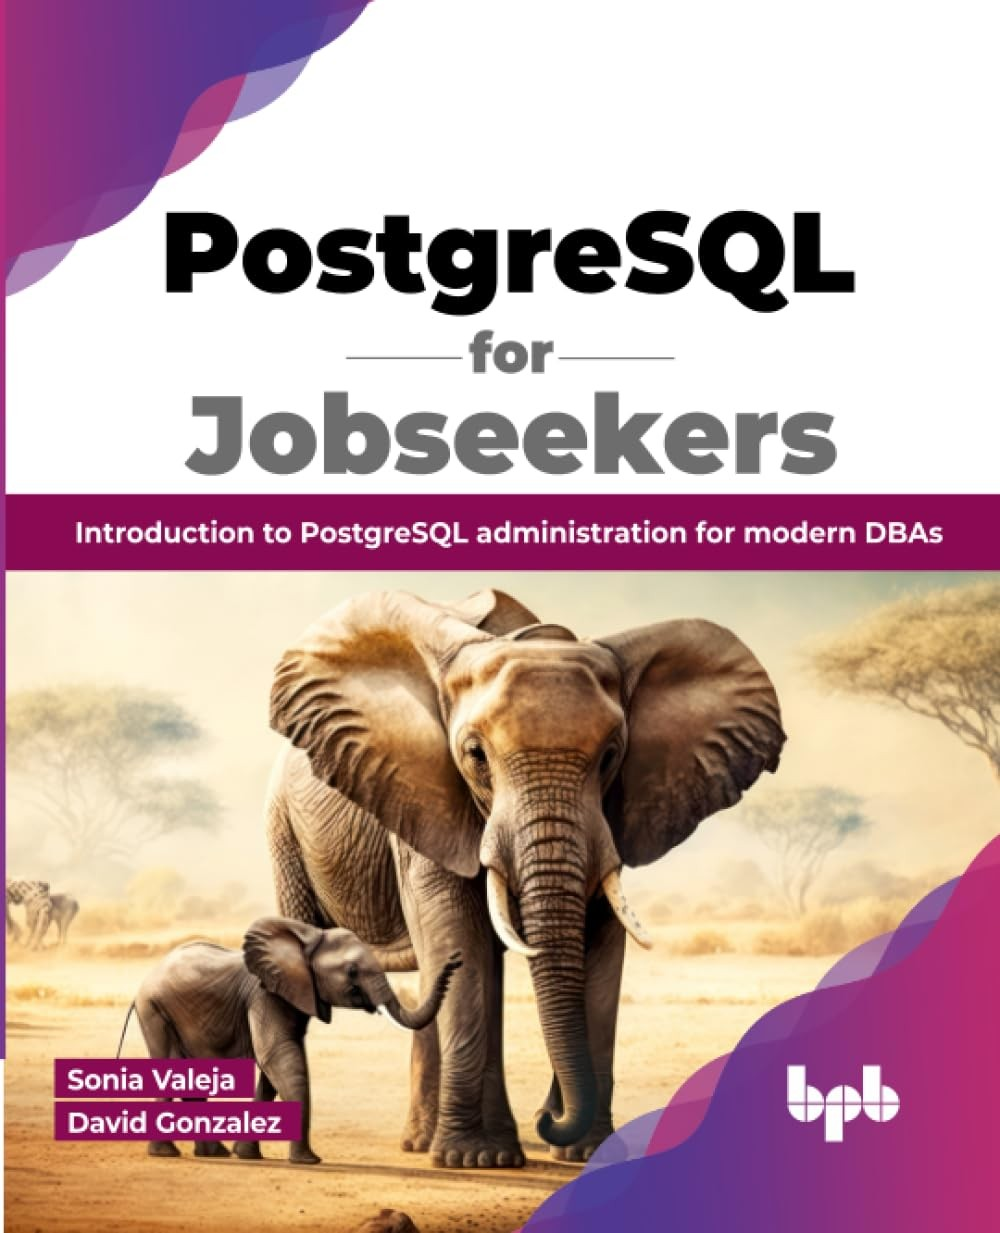
\includegraphics[width=0.35\textwidth]{figures/book_cover}\\
    \vspace{2mm}
    {
        \scriptsize
        Content has been extracted from \textit{PostgreSQL for Jobseekers (Chapter 13)}, by Sonia Valeja and David Gonzales, 2023.  Visit \url{https://bpbonline.com/products/postgresql-for-jobseekers}.\\
    }
\end{frame}

% Introduction
\section{Introduction}

\begin{frame}{Introduction to Performance Tuning}
  \justifying
  Any \textbf{Relational Database Management System (RDBMS)} intends to resolve user queries as quickly as possible, and PostgreSQL is no exception.
  Keeping PostgreSQL performant is one of the main goals for Database Administrators (DBAs).

  \vspace{0.3cm}
  Now, we will dive into the \textbf{performance tuning topics}. We will learn about the basic concepts and components involved in database tuning and some best practices we can use as an initial guide.
\end{frame}

\begin{frame}{Introduction to Performance Tuning}
    \begin{itemize}
        \item PostgreSQL aims to resolve queries as quickly as possible.
        \item Performance tuning is a critical aspect of database administration.
        \item This presentation covers key topics including: indexes, statistics, query planning, and best practices.
    \end{itemize}
\end{frame}

% Indexes
\section{Indexes}

\begin{frame}{Indexes}
    \begin{itemize}
        \item Indexes help locate data efficiently, similar to a book index.
        \item Types of indexes:
        \begin{itemize}
            \item B-tree (default, supports range queries)
            \item Hash (optimized for equality comparisons)
            \item GiST and SP-GiST (used for geometric data)
            \item GIN (for arrays and full-text search)
            \item BRIN (efficient for large datasets with ordered values)
        \end{itemize}
    \end{itemize}
\end{frame}


\begin{frame}[fragile]{Indexes}
    \begin{minted}
    [tabsize=4, obeytabs, frame=lines, framesep=2mm, baselinestretch=1.2, bgcolor=LightGray, fontsize=\scriptsize]{text}
CREATE [ UNIQUE ] INDEX [ CONCURRENTLY ] [ [ IF NOT EXISTS ] name ] ON
[ ONLY ] table_name [ USING method ]
    ( { column_name | ( expression ) } [ COLLATE collation ] [ opclass
    [ ( opclass_parameter = value [, ... ] ) ] ] [ ASC | DESC ] [ NULLS
    { FIRST | LAST } ] [, ...] )
    [ INCLUDE ( column_name [, ...] ) ]
    [ NULLS [ NOT ] DISTINCT ]
    [ WITH ( storage_parameter [= value] [, ... ] ) ]
    [ TABLESPACE tablespace_name ]
    [ WHERE predicate ]
    \end{minted}


    \begin{minted}
    [tabsize=4, obeytabs, frame=lines, framesep=2mm, baselinestretch=1.2, bgcolor=LightGray, fontsize=\scriptsize]{text}
CREATE INDEX <schema_name>.<index_name> on <table_name> (<column/column-list>)
    \end{minted}
\end{frame}

\begin{frame}{Index Creation Notes}
  \begin{itemize}
    \item \textbf{CREATE} and \textbf{DROP} indexes are not online activities by default.
          The table is locked for modifications during these operations.

    \item Read operations can still be performed during index creation/modification
          if the \texttt{CONCURRENTLY} keyword is used.

    \item Multi-column indexes can be created to improve performance on queries
          involving multiple columns.

    \item When creating multi-column indexes, ensure the column order matches
          the order used in the query’s \texttt{WHERE} clause.
  \end{itemize}
\end{frame}


% Reindexing
\begin{frame}{Reindexing}
    \begin{itemize}
        \item Rebuilding an index can help maintain performance.
        \item Command: \texttt{REINDEX INDEX <index-name>}
        \item Use \texttt{CONCURRENTLY} to rebuild without locking writes.
    \end{itemize}
\end{frame}

\begin{frame}[fragile]{Indexes}
    \begin{minted}
    [tabsize=4, obeytabs, frame=lines, framesep=2mm, baselinestretch=1.2, bgcolor=LightGray, fontsize=\scriptsize]{text}
REINDEX [ ( option [, ...] ) ] { INDEX | TABLE | SCHEMA | DATABASE | SYSTEM }
[ CONCURRENTLY ] name
    \end{minted}

    where option can be one of:
    \begin{minted}
    [tabsize=4, obeytabs, frame=lines, framesep=2mm, baselinestretch=1.2, bgcolor=LightGray, fontsize=\scriptsize]{text}
CONCURRENTLY [ boolean ] – Reindex can be created concurrently online
TABLESPACE new_tablespace – Reindexing could be done in tablespace new
VERBOSE [ boolean ] – Logs will be printed while reindexing
    \end{minted}
\end{frame}

\begin{frame}{Automatic Index Creation}
  \begin{itemize}
    \item When a \textbf{Primary Key} or \textbf{Unique Key} constraint is created, PostgreSQL automatically creates indexes on those columns.
    \item These columns are frequently used for fetching data in queries.
    \item It is also a good practice to create indexes on:
      \begin{itemize}
        \item Columns used in \texttt{WHERE} clauses.
        \item Foreign key columns in child tables (often used in \texttt{JOIN} conditions).
      \end{itemize}
  \end{itemize}
\end{frame}

\begin{frame}{Index Usage Over Time}
  \begin{itemize}
    \item For small databases, default indexes (Primary Key, Unique) are often enough.
    \item As data grows, queries may slow down, making additional indexes useful.
    \item Use \texttt{EXPLAIN PLAN} to verify whether queries benefit from indexes.
    \item Indexes are essential building blocks for improving performance of:
      \begin{itemize}
        \item Reporting queries.
        \item \texttt{SELECT} queries requiring faster execution.
      \end{itemize}
  \end{itemize}
\end{frame}

\begin{frame}{Indexes and Query Performance}
  \begin{itemize}
    \item Indexes can also improve the performance of \texttt{INSERT}, \texttt{UPDATE}, and \texttt{DELETE} queries with \texttt{WHERE} conditions.
    \item The \texttt{ANALYZE} command keeps index statistics up to date.
    \item Updated statistics ensure the query planner chooses the most efficient execution plan.
  \end{itemize}
\end{frame}

\begin{frame}{Indexes and Expressions}
  \begin{itemize}
    \item An index column does not need to be a raw table column.
    \item It can be a \textbf{function} or \textbf{scalar expression} computed from one or more columns.
    \item This allows PostgreSQL to optimize queries involving computed values.
    \item Example: concatenate \texttt{first\_name} and \texttt{last\_name}.
  \end{itemize}

  \vspace{0.3cm}
  \begin{exampleblock}{Example Query}
  \scriptsize
  \texttt{SELECT * FROM people \\
  \hspace{0.3cm}WHERE (first\_name || ' ' || last\_name) = 'John Smith';}
  \end{exampleblock}
\end{frame}

\begin{frame}{Expression Index Benefits}
  \begin{itemize}
    \item Create an index on the same expression used in queries:
    \begin{exampleblock}{Example Index}
    \scriptsize
    \texttt{CREATE INDEX people\_names \\
    \hspace{0.3cm}ON people ((first\_name || ' ' || last\_name));}
    \end{exampleblock}
    \item The system treats the expression as a normal indexed column.
    \item Search speed becomes equivalent to simple index lookups.
    \item Useful when retrieval speed is more important than insertion or update speed.
    \item Metadata views \texttt{pg\_index} and \texttt{pg\_indexes} provide details on schema, index name, and more.
  \end{itemize}
\end{frame}

% Statistics
\section{Statistics}

\begin{frame}{Statistics in PostgreSQL}
  \begin{itemize}
    \item Statistics are \textbf{metadata} — data about the data.
    \item The \textbf{query planner} relies on statistics to determine the fastest and cheapest execution path.
    \item Collected statistics guide how PostgreSQL retrieves the required data efficiently.
    \item Two main types of statistics exist, maintained by different components.
  \end{itemize}
\end{frame}

\begin{frame}{Types of Statistics}
  \begin{itemize}
    \item \textbf{Server activity statistics}
      \begin{itemize}
        \item Collected by the \textbf{stats collector} background process.
        \item Includes: table/index access counts, user session information.
        \item Used mainly by DBAs to verify system state.
      \end{itemize}
    \vspace{0.3cm}
    \item \textbf{Data distribution statistics}
      \begin{itemize}
        \item Collected by \texttt{ANALYZE} or \texttt{VACUUM ANALYZE}, manually or via autovacuum.
        \item Provides data distribution details for the planner.
        \item Directly impacts query execution decisions.
      \end{itemize}
  \end{itemize}
\end{frame}

\begin{frame}{System Catalogs for Statistics}
  \begin{itemize}
    \item \textbf{pg\_class}:
      Stores statistics about number of tuples (rows), disk blocks, and object identity details.

    \item \textbf{pg\_statistics}:
      Contains selectivity information per table column.
      \begin{itemize}
        \item One or two rows per column (depending on inheritance).
        \item Intended for system use, but \texttt{pg\_stats} view provides a user-friendly version.
      \end{itemize}

    \item \textbf{pg\_statistics\_ext\_data}:
      Stores additional information for extended statistics objects on sets of columns.
  \end{itemize}
\end{frame}

\begin{frame}[fragile]{Statistics in \texttt{pg\_class}}
    \begin{minted}
    [tabsize=4, obeytabs, frame=lines, framesep=2mm, baselinestretch=1.2, bgcolor=LightGray, fontsize=\scriptsize]{sql}
SELECT
    relname AS relation_name,
    relkind AS relation_kind,
    reltuples AS relation_tuples,
    relpages AS relation_pages,
    pg_size_pretty(pg_relation_size(oid)) AS relation_size
FROM
    pg_class
WHERE
    relname LIKE 'address%'
    AND relkind IN ('r', 'i');
    \end{minted}
\end{frame}

\begin{frame}[fragile]{Statistics in \texttt{pg\_class}}
    \begin{minted}
    [tabsize=4, obeytabs, frame=lines, framesep=2mm, baselinestretch=1.2, bgcolor=LightGray, fontsize=\scriptsize]{text}
-[ RECORD 1 ]---+-------------
relation_name| address
relation_kind| r
relation_tuples | 603
relation_pages| 8
relation_size| 64 kB
-[ RECORD 2 ]---+-------------
relation_name| address_pkey
relation_kind| i
relation_tuples | 603
relation_pages| 4
relation_size| 32 kB
    \end{minted}
\end{frame}

\begin{frame}[fragile]{Statistics in \texttt{pg\_statistics} (\texttt{pg\_stats} view)}
    \begin{minted}
    [tabsize=4, obeytabs, frame=lines, framesep=2mm, baselinestretch=1.2, bgcolor=LightGray, fontsize=\scriptsize]{sql}
SELECT
    attname AS column_name,
    n_distinct AS distinct_rate,
    array_to_string(most_common_vals, E'\n') AS most_common_values,
    array_to_string(most_common_freqs, E'\n') AS most_common_frequencies
FROM
    pg_stats
WHERE tablename = 'address'
    AND attname = 'postal_code';
    \end{minted}
\end{frame}

\begin{frame}[fragile]{Statistics in \texttt{pg\_class}}
    \begin{minted}
    [tabsize=4, obeytabs, frame=lines, framesep=2mm, baselinestretch=1.2, bgcolor=LightGray, fontsize=\scriptsize]{text}
-[ RECORD 1 ]---------------+-------------
column_name                 | postal_code
distinct_rate               | 0.9900498
most_common_values          |   +
                            | 22474+
                            | 52137+
                            | 9668
most_common_frequencies     | 0.006633499 +
                            | 0.0033167496+
                            | 0.0033167496+
                            | 0.0033167496
    \end{minted}
\end{frame}

\begin{frame}{Extended Statistics in PostgreSQL}
  \begin{itemize}
    \item Standard statistics track rows, disk space, and column selectivity.
    \item Some queries involve correlations across multiple columns, which single-column stats cannot capture.
    \item PostgreSQL supports \textbf{extended statistics}, but they are not gathered by default.
    \item DBAs must define them explicitly using:
      \begin{itemize}
        \item \texttt{CREATE STATISTICS} command.
      \end{itemize}
    \item Goal: describe correlations between columns to improve the planner’s row estimations.
    \item Requires human intervention since relationships depend on the database model.
  \end{itemize}
\end{frame}

\begin{frame}{Extended Statistics in PostgreSQL}
    \centering
    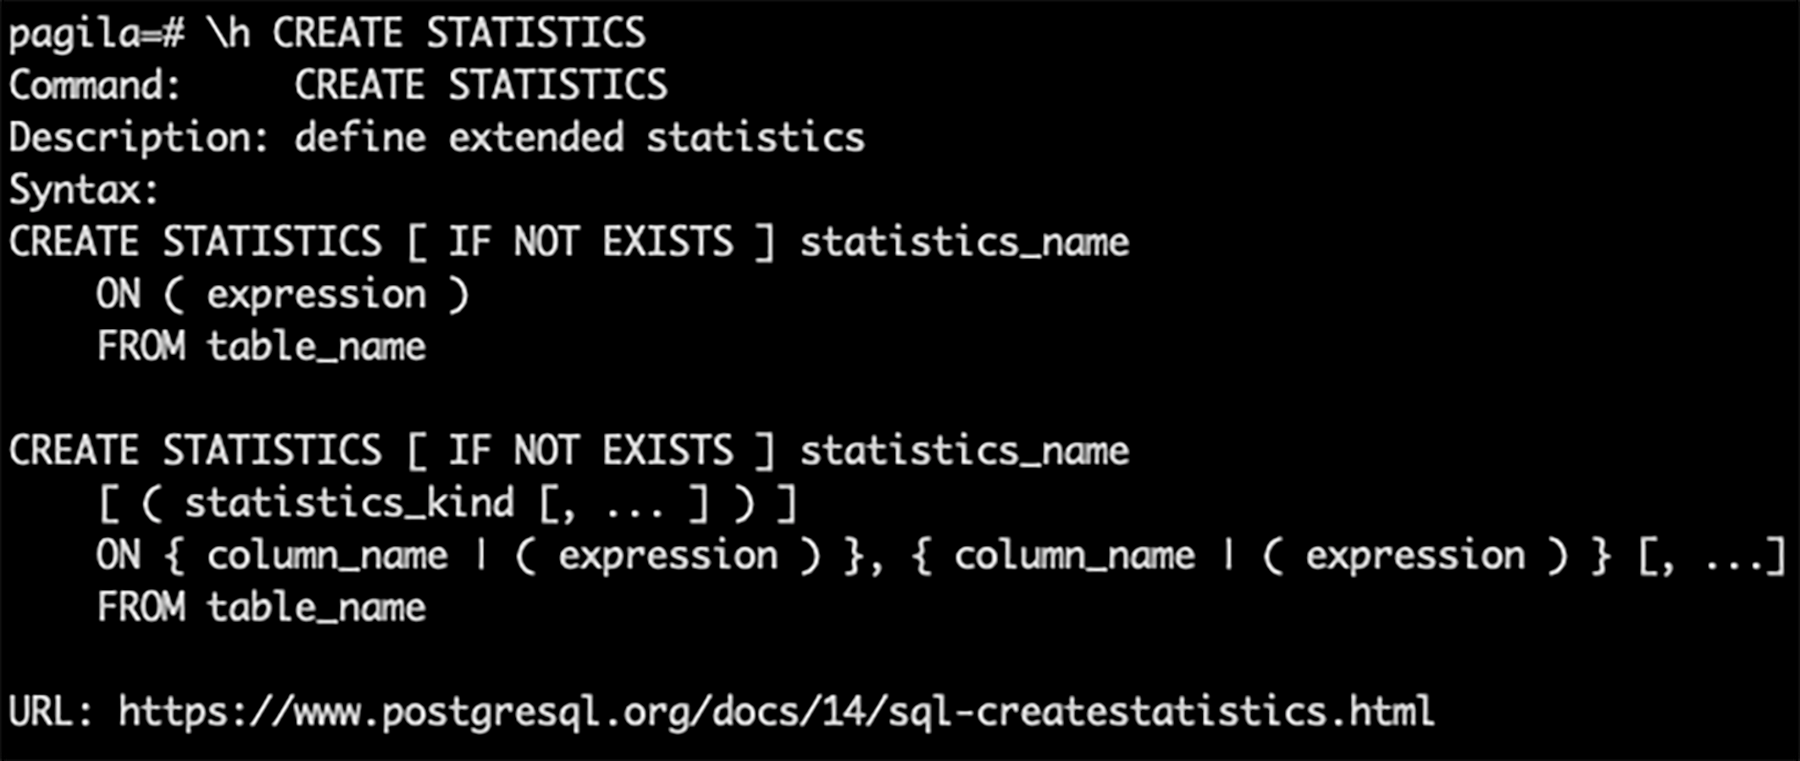
\includegraphics[width=0.95\textwidth]{figures/create_stats}
\end{frame}


\begin{frame}{Extended Statistics in PostgreSQL}
    \Large \textbf{Homework}:
    Summarize sections about the three types of extended statistics\footnote{page 243 in the textbook}, each covering a distinct kind of column values correlation:
    \begin{enumerate}
        \item Functional dependencies.
        \item Number of distinct values counts.
        \item Most common values list.
    \end{enumerate}
\end{frame}

% EXPLAIN PLAN
\begin{frame}{EXPLAIN PLAN}
    \begin{itemize}
        \item Used to analyze query execution plans.
        \item Syntax: \texttt{EXPLAIN ANALYZE <query>}
        \item Helps identify if indexes are used or if sequential scans occur.
    \end{itemize}
\end{frame}

\begin{frame}[fragile]{EXPLAIN PLAN}
    \begin{minted}
    [tabsize=4, obeytabs, frame=lines, framesep=2mm, baselinestretch=1.2, bgcolor=LightGray, fontsize=\scriptsize]{text}
EXPLAIN [ ( option [, ...] ) ] statement
EXPLAIN [ ANALYZE ] [ VERBOSE ] statement
    \end{minted}

    where option can be one of:
    \begin{minted}
    [tabsize=4, obeytabs, frame=lines, framesep=2mm, baselinestretch=1.2, bgcolor=LightGray, fontsize=\scriptsize]{text}
ANALYZE [ boolean ]
VERBOSE [ boolean ]
COSTS [ boolean ]
SETTINGS [ boolean ]
BUFFERS [ boolean ]
WAL [ boolean ]
TIMING [ boolean ]
SUMMARY [ boolean ]
FORMAT { TEXT | XML | JSON | YAML }
    \end{minted}
\end{frame}


\begin{frame}{In action}
    \centering
    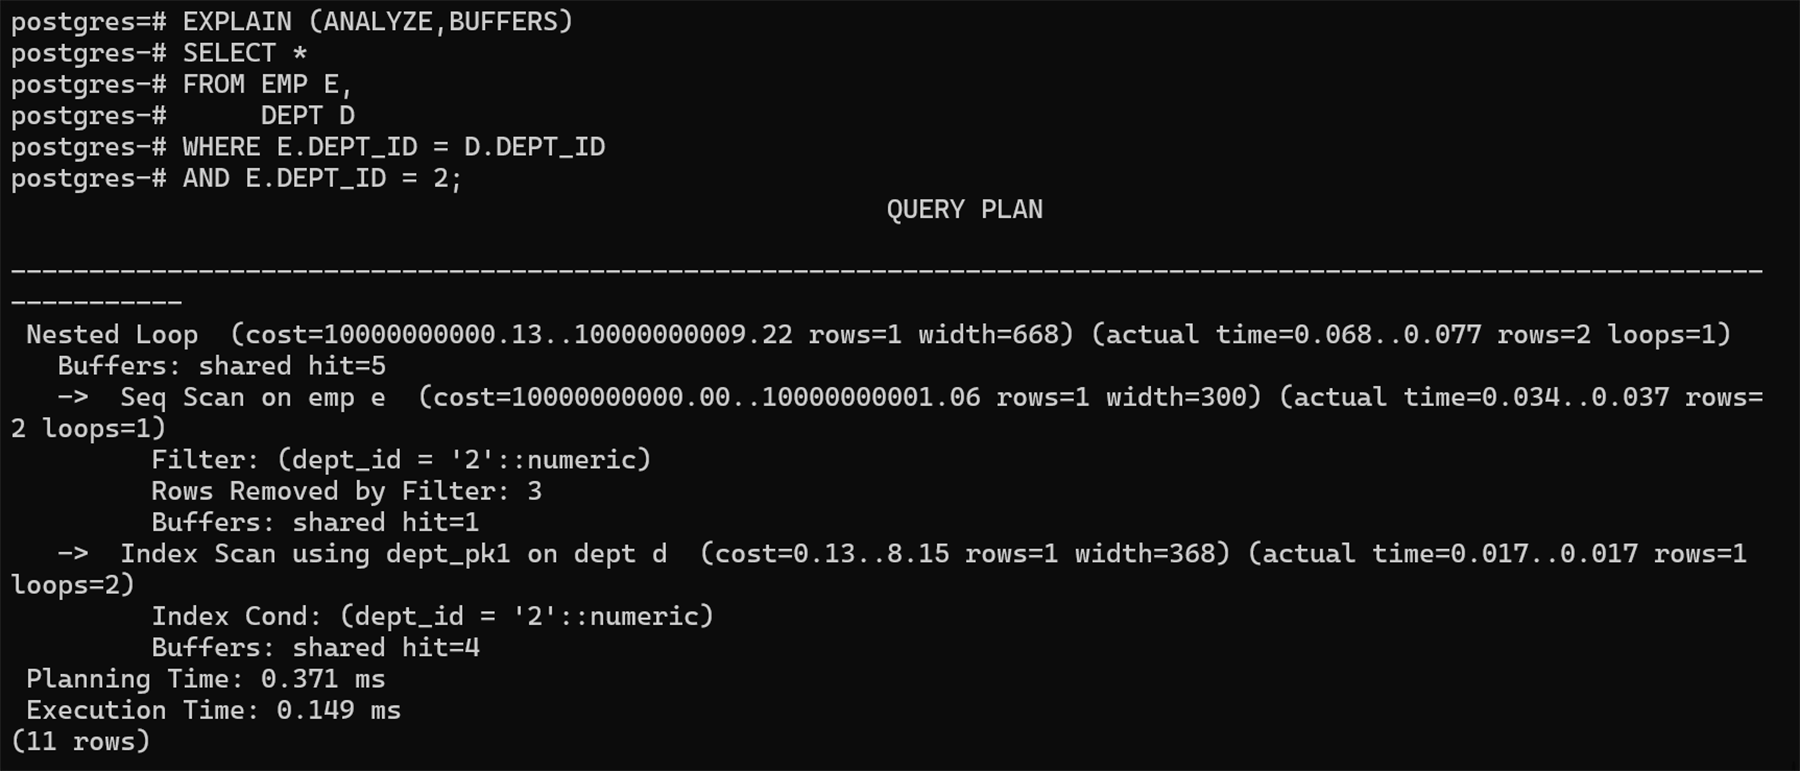
\includegraphics[width=0.95\textwidth]{figures/explain1}
\end{frame}


\begin{frame}{In action}
    \centering
    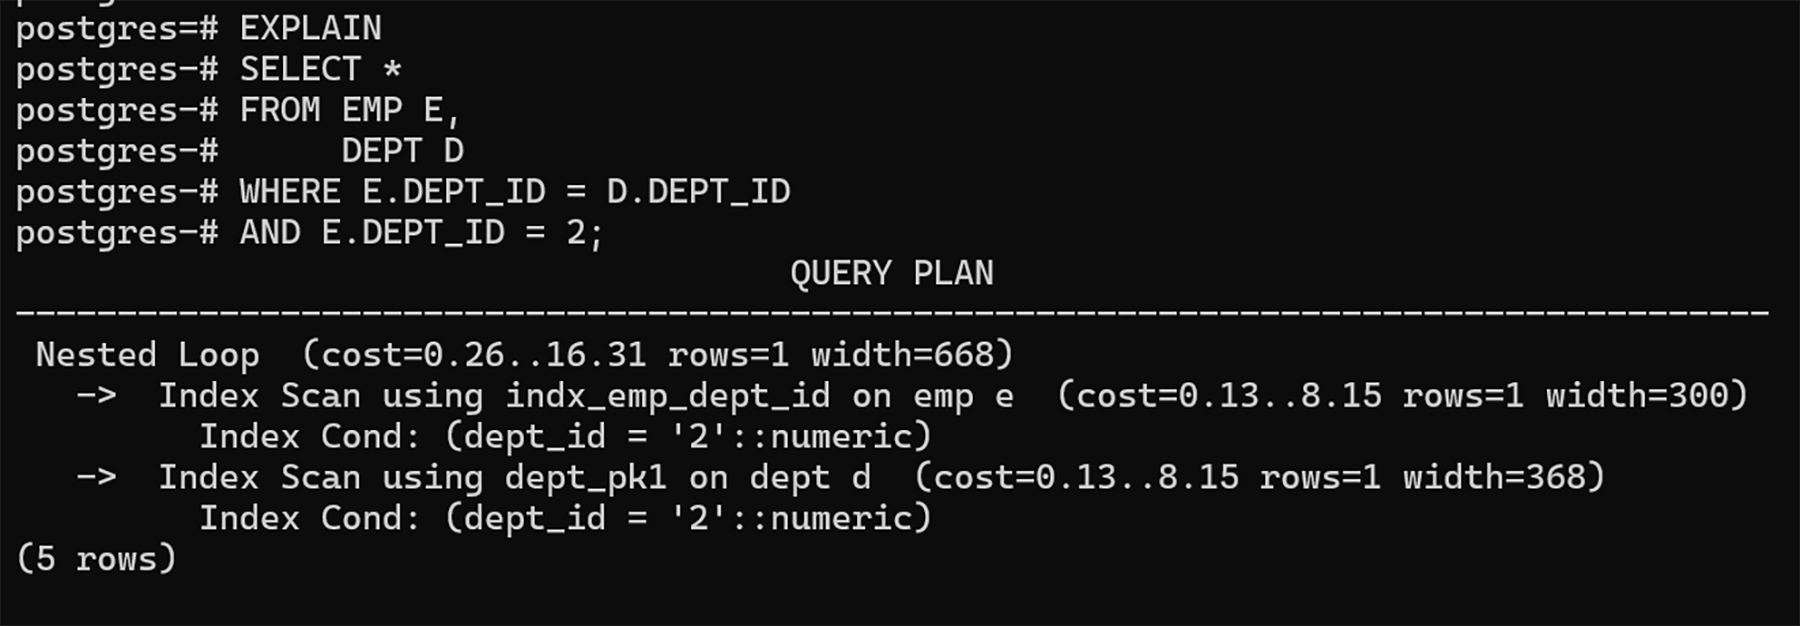
\includegraphics[width=0.95\textwidth]{figures/explain2}
\end{frame}

% Best Practices
\section{Best Practices}

\begin{frame}{Best Practices for Performance Tuning}
    \begin{itemize}
        \item Adjust key parameters in \texttt{postgresql.conf}:
        \begin{itemize}
            \item \texttt{shared\_buffers}: Set to 15-25\% of RAM.
            \item \texttt{work\_mem}: Allocate sufficient memory for sorting.
            \item \texttt{effective\_cache\_size}: Set to 50-75\% of RAM.
            \item \texttt{autovacuum}: Ensure it is enabled for table maintenance.
        \end{itemize}
        \item Regularly analyze and vacuum tables.
        \item Use indexes strategically to avoid unnecessary overhead.
    \end{itemize}
\end{frame}

\begin{frame}{Best Practices for Performance Tuning}
    \centering
    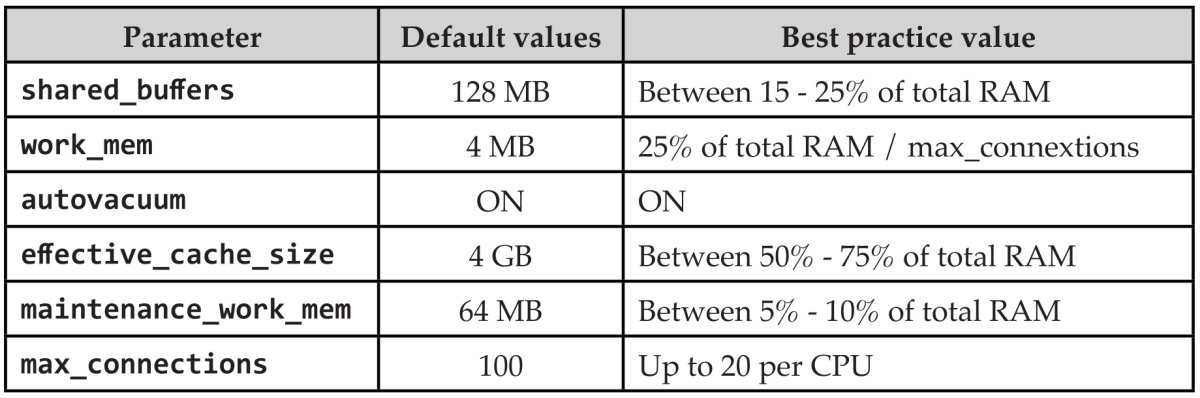
\includegraphics[width=\textwidth]{figures/best}
\end{frame}

\section*{Takeaways}

% Tim Duncan's Top 5 Fundamental Takeaways of the Today's Class
\begin{frame}{TDT5FTOTC}
    \centering
    
\includegraphics[height=0.9\textheight]{figures/tim.png}
\end{frame}

\begin{frame}{TDT5FTOTC}
    \pause
    \begin{itemize}
        \item[5] \textbf{Indexes are the foundation of query performance}, with PostgreSQL creating them automatically for Primary and Unique Keys while DBAs should add them strategically for foreign keys and frequent WHERE clauses. \pause

        \item[4] \textbf{Indexes improve SELECT performance} but add overhead to writes, so their effectiveness should be checked with \texttt{EXPLAIN PLAN} and maintained using \texttt{ANALYZE}. \pause

        \item[3] PostgreSQL relies on \textbf{statistics as metadata} for query planning, with server activity statistics and data distribution statistics stored in catalogs like \texttt{pg\_class}, \texttt{pg\_stats}, and \texttt{pg\_statistics\_ext\_data}. \pause

        \item[2] \textbf{Extended statistics} defined with \texttt{CREATE STATISTICS} improve multi-column query optimization by capturing functional dependencies, distinct value counts, and common value lists. \pause

        \item[1] \textbf{Best practices} include tuning key parameters in \texttt{postgresql.conf}, keeping autovacuum enabled, running \texttt{ANALYZE}/\texttt{VACUUM} regularly, and using indexes strategically.
    \end{itemize}
\end{frame}

\begin{frame}{Database Administration: Backup and Restore.}
    \centering
    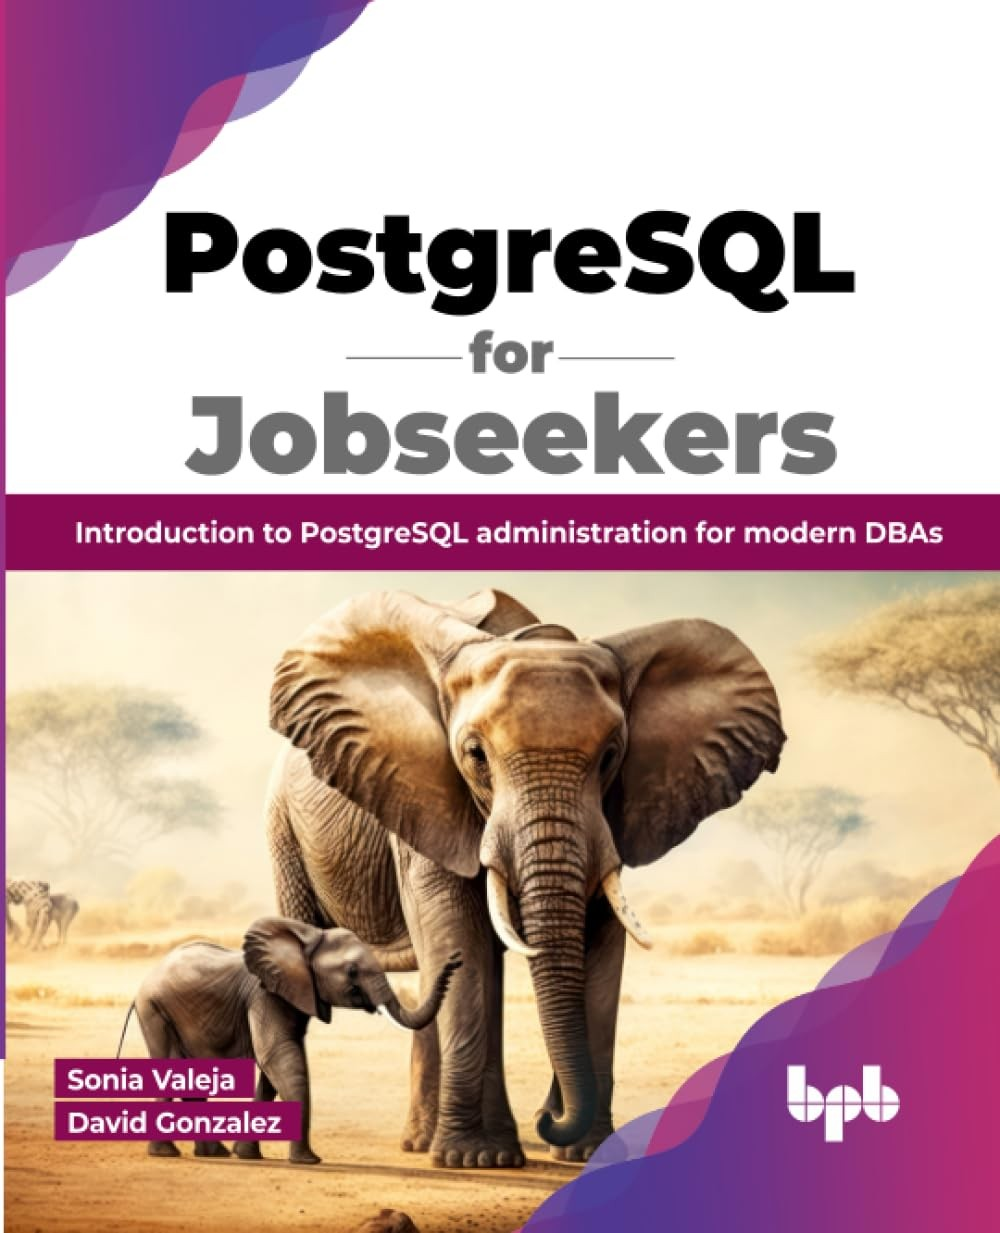
\includegraphics[width=0.35\textwidth]{figures/book_cover}\\
    \vspace{2mm}
    {
        \scriptsize
        Content has been extracted from \textit{PostgreSQL for Jobseekers (Chapter 13)}, by Sonia Valeja and David Gonzales, 2023.  Visit \url{https://bpbonline.com/products/postgresql-for-jobseekers}.\\
    }
\end{frame}

\end{document}
